% SOURCE_AUTHORITY: sga5_fr_workpass.tex, lines 1989--2142 (LF-normalized unit).
% SOURCE_SHA256: 791F4EFFC5E02832D5D77ED03518C8156D6F07E4C8238B03545DB93D883FBB28
\subsection*{2.1}
Sejam $f:X\to Y$ um $S$-morfismo, $P\in\ob D(Y)$, $Q\in\ob D^{+}(Y)$. A flecha canônica evidente no nível dos complexos
\[
f^{*}\mathcal Hom^{\bullet}(P,Q)\longrightarrow\mathcal Hom^{\bullet}(f^{*}P,f^{*}Q)
\]
fornece por derivação uma flecha canônica
\begin{equation}\tag{2.1.1}
f^{*}\uRHom(P,Q)\longrightarrow\uRHom(f^{*}P,f^{*}Q).
\end{equation}
Sejam $L\in\ob D(X)$, $M\in\ob D^{+}(X)$. Ponhamos
\begin{equation}\tag{2.1.2}
\Hom_f^{(i,j)}((L,M),(P,Q))=\Hom_f^{(i)}(L,P)\times\Hom_f^{(j)}(M,Q),
\end{equation}
com as notações de 1.4. Para $(u,v)\in\Hom_f^{(2,1)}((L,M),(P,Q))$ define-se
\begin{equation}\tag{2.1.3}
\uRHom(u,v)\in\Hom_f^{(1)}(\uRHom(L,M),\uRHom(P,Q))
\end{equation}
compondo 2.1.1 com a flecha $\uRHom(f^{*}P,f^{*}Q)\to\uRHom(L,M)$ definida por $u$ e $v$. Para $L=f^{*}P$, $Q=f_{*}M$, $u$ (resp. $v$) dada pela identidade de $L$ (resp. $Q$), $\uRHom(u,v)$ é o isomorfismo de ``dualidade trivial''
\begin{equation}\tag{2.1.4}
\uRHom(P,f_{*}M)\xrightarrow{\sim}f_{*}\uRHom(f^{*}P,M).
\end{equation}
Para $(u,v)\in\Hom_f^{(3,4)}((L,M),(P,Q))$, define-se
\begin{equation}\tag{2.1.5}
\uRHom(u,v)\in\Hom_f^{(1)}(\uRHom(L,M),\uRHom(P,Q))
\end{equation}
como a composta das flechas
\[
\uRHom(P,Q)\xrightarrow{a}\uRHom(f_{!}L,Q)\xrightarrow{b}f_{*}\uRHom(L,f^{!}Q)\xrightarrow{c}f_{*}\uRHom(L,M),
\]
onde $a$ (resp. $c$) é definida por $u$ (resp. $v$), e $b$ é o inverso do isomorfismo de dualidade (SGA~4~XVIII~3.1.9.6).

Deduz-se facilmente das definições que a formação de $\uRHom(u,v)$ é compatível com a composição: para $(u,v)$, $(u',v')$ componíveis e de tipo $(2,1)$ (resp. $(3,4)$), tem-se
\begin{equation}\tag{2.1.6}
\uRHom(u'u,v'v)=\uRHom(u',v')\,\uRHom(u,v).
\end{equation}

\subsection*{2.2}
Seja $X$ um $S$-esquema. Recordemos que, para $L\in\ob D^{-}(X)$, $M\in\ob D(X)$, $N\in\ob D^{+}(X)$, tem-se o isomorfismo de adjunção (``querido por Cartan'', como diz Grothendieck)
\begin{equation}\tag{2.2.1}
\Hom(L\otimes^{L}M,N)=\Hom(L,\uRHom(M,N)).
\end{equation}
Para $E\in\ob D^{-}(X)$, $F\in\ob D^{+}(X)$, a flecha identidade de $\uRHom(E,F)$ define, mediante 2.2.1, uma flecha
\begin{equation}\tag{2.2.2}
E\otimes^{L}\uRHom(E,F)\longrightarrow F,
\end{equation}
chamada \emph{flecha de avaliação}: deriva da flecha no nível dos complexos
\[
\mathcal Hom^{\bullet}(E,F)\otimes E\longrightarrow F,
\qquad f\otimes x\longmapsto f(x).
\]
Sejam, para $i=1,2$, $E_i,F_i\in\ob D_{\ctf}(X)$. Por adjunção (2.2.1), a flecha
\[
E_1\otimes^{L}E_2\otimes^{L}\uRHom(E_1,F_1)\otimes^{L}\uRHom(E_2,F_2)\longrightarrow F_1\otimes^{L}F_2,
\]
composta de um isomorfismo de simetria e do produto tensorial das flechas de avaliação relativas a $(E_1,F_1)$ e $(E_2,F_2)$, fornece uma flecha
\begin{equation}\tag{2.2.3}
\uRHom(E_1,F_1)\otimes^{L}\uRHom(E_2,F_2)\longrightarrow\uRHom(E_1\otimes^{L}E_2,F_1\otimes^{L}F_2).
\end{equation}
Sejam, para $i=1,2$, $X_i$ um $S$-esquema, $X=X_1\times_SX_2$, $p_i:X\to X_i$ a projeção canônica, $E_i,F_i\in\ob D_{\ctf}(X_i)$, $E=E_1\otimes^{L}_{S}E_2$, $F=F_1\otimes^{L}_{S}F_2$. Tem-se uma flecha canônica
\begin{equation}\tag{2.2.4}
\uRHom(E_1,F_1)\otimes^{L}_{S}\uRHom(E_2,F_2)\longrightarrow\uRHom(E,F),
\end{equation}
composta do produto tensorial das flechas $p_i^{*}\uRHom(E_i,F_i)\to\uRHom(p_i^{*}E_i,p_i^{*}F_i)$ e de 2.2.3 para $(p_i^{*}E_i,p_i^{*}F_i)$.

\subsection*{Proposição 2.3}
A flecha 2.2.4 é um isomorfismo.

Por localização e devissage, reduzimo-nos a $E_i=f_{i!}A_{U_i}$ para $f_i:U_i\to X_i$ étale. Têm-se isomorfismos canônicos (dualidade)
\begin{equation}\tag{1}
\uRHom(f_{i!}A_{U_i},F_i)\xrightarrow{\sim}f_{i*}f_i^{*}F_i,
\qquad
\uRHom(E,F)\xrightarrow{\sim}f_{*}f^{*}F\quad(f=f_1\times_S f_2).
\end{equation}
Levando em conta a fórmula de Künneth 1.6.4, basta, para concluir, verificar que esses isomorfismos tornam comutativo o quadrado
\begin{equation}\tag{2}
\begin{tikzcd}[column sep=large,row sep=large]
\uRHom(f_{1!}A_{U_1},F_1)\otimes^{L}_{S}\uRHom(f_{2!}A_{U_2},F_2) \arrow[r,"2.2.3"] \arrow[d,"\sim"'] & \uRHom(f_{!}A_U,F) \arrow[d,"\sim"]\\
f_{1*}f_1^{*}F_1\otimes^{L}_{S}f_{2*}f_2^{*}F_2 \arrow[r,"1.6.4"'] & f_{*}f^{*}F,
\end{tikzcd}
\end{equation}
onde $U=U_1\times_S U_2$. Agora, como $f_i$ é étale, o isomorfismo (1) relativo a $f_i$ (resp. $f$) é o adjunto da flecha composta
\begin{equation}\tag{3}
f_i^{*}\uRHom(f_{i!}A_{U_i},F_i)\xrightarrow{\sim}\uRHom(f_i^{*}f_{i!}A_{U_i},f_i^{*}F_i)\longrightarrow f_i^{*}F_i,
\end{equation}
onde a segunda flecha se deduz da adjunção $A_{U_i}\to f_i^{*}f_{i!}A_{U_i}$ (resp. da flecha composta análoga com $f$). A comutatividade de (2) equivale à do quadrado
\begin{equation}\tag{4}
\begin{tikzcd}[column sep=large,row sep=large]
f_1^{*}\uRHom(f_{1!}A_{U_1},F_1)\otimes^{L}_{S}f_2^{*}\uRHom(f_{2!}A_{U_2},F_2) \arrow[r] \arrow[d] & f^{*}\uRHom(f_{!}A_U,F) \arrow[d]\\
f_1^{*}F_1\otimes^{L}_{S}f_2^{*}F_2 \arrow[r,"\sim"] & f^{*}F,
\end{tikzcd}
\end{equation}
onde as flechas verticais são dadas por (3). Ora, a comutatividade de (4) deduz-se do fato de que 2.2.3 é funtorial em $E_i$ e se reduz à identidade para $E_i=A$, daí resultando a proposição.

\subsection*{2.4}
Sejam, para $i=1,2$, $f_i:X_i\to Y_i$ um $S$-morfismo,
\[
f=f_1\times_S f_2:X\to Y,
\]
$E_i,F_i\in\ob D_{\ctf}(X_i)$, $P_i,Q_i\in\ob D_{\ctf}(Y_i)$,
\[
E=E_1\otimes^{L}_{S}E_2,
\quad F=F_1\otimes^{L}_{S}F_2,
\quad P=P_1\otimes^{L}_{S}P_2,
\quad Q=Q_1\otimes^{L}_{S}Q_2.
\]
Consideremos o diagrama
\begin{equation}\tag{2.4.0}
\resizebox{0.96\textwidth}{!}{%
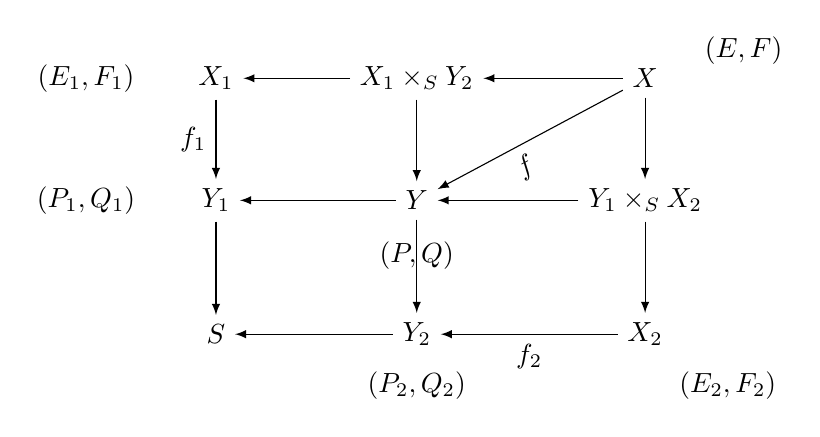
\begin{tikzpicture}[>=latex,baseline=(current bounding box.center)]
\node (EF1) at (-5.2,2.0) {$(E_1,F_1)$};
\node (X1)  at (-3.55,2.0) {$X_1$};
\node (X1Y2) at (-1.0,2.0) {$X_1\times_S Y_2$};
\node (X) at (1.9,2.0) {$X$};
\node (EF) at (3.15,2.35) {$(E,F)$};
\node (PQ1) at (-5.2,0.45) {$(P_1,Q_1)$};
\node (Y1) at (-3.55,0.45) {$Y_1$};
\node (Y) at (-1.0,0.45) {$Y$};
\node (Y1X2) at (1.9,0.45) {$Y_1\times_S X_2$};
\node (S) at (-3.55,-1.25) {$S$};
\node (Y2) at (-1.0,-1.25) {$Y_2$};
\node (X2) at (1.9,-1.25) {$X_2$};
\node (PQ) at (-1.0,-0.25) {$(P,Q)$};
\node (PQ2) at (-1.0,-1.9) {$(P_2,Q_2)$};
\node (EF2) at (2.95,-1.9) {$(E_2,F_2)$};
\draw[->] (X1Y2) -- (X1);
\draw[->] (X) -- (X1Y2);
\draw[->] (X1) -- node[left] {$f_1$} (Y1);
\draw[->] (X1Y2) -- (Y);
\draw[->] (X) -- (Y1X2);
\draw[->] (X) -- node[below,sloped,pos=.58] {$f$} (Y);
\draw[->] (Y) -- (Y1);
\draw[->] (Y1X2) -- (Y);
\draw[->] (Y1) -- (S);
\draw[->] (Y) -- (Y2);
\draw[->] (Y1X2) -- (X2);
\draw[->] (Y2) -- (S);
\draw[->] (X2) -- node[below] {$f_2$} (Y2);
\end{tikzpicture}}
\end{equation}
Fixemos $(u_1,v_1)\in\Hom_{f_1}^{(3,4)}((E_1,F_1),(P_1,Q_1))$, $(u_2,v_2)\in\Hom_{f_2}^{(2,1)}((E_2,F_2),(P_2,Q_2))$ (notações de 2.1.2 e 1.4). Por 1.8, de $(u_i,v_i)$ deduz-se um quadrado
\begin{equation}\tag{2.4.1}
\resizebox{0.92\textwidth}{!}{%
\begin{tikzcd}[ampersand replacement=\&,column sep=huge,row sep=large]
(E_1\otimes^L_S P_2,F_1\otimes^L_S Q_2)
  \arrow[d,"{(u_1\otimes^L_S P_2,\,v_1\otimes^L_S Q_2)}"']
  \& (E,F) \arrow[l,"{(E_1\otimes^L_S u_2,\,F_1\otimes^L_S v_2)}"'] \arrow[d,"{(u_1\otimes^L_S E_2,\,v_1\otimes^L_S F_2)}"] \\
(P,Q)
  \& (P_1\otimes^L_S E_2,Q_1\otimes^L_S F_2) \arrow[l,"{(P_1\otimes^L_S u_2,\,Q_1\otimes^L_S v_2)}"']
\end{tikzcd}}
\end{equation}
onde as flechas verticais (resp. horizontais) são de tipo $(3,4)$ (resp. $(2,1)$).

Agora podemos enunciar a compatibilidade principal deste número, que desempenhará um papel essencial na verificação da fórmula de Lefschetz--Verdier.
